\documentclass{article}

% Language setting
% Replace `english' with e.g. `spanish' to change the document language
\usepackage[english]{babel}

% Set page size and margins
% Replace `letterpaper' with `a4paper' for UK/EU standard size
\usepackage[letterpaper,top=2cm,bottom=2cm,left=3cm,right=3cm,marginparwidth=1.75cm]{geometry}

% Useful packages
\usepackage{amsmath}
\usepackage{amsfonts}
\usepackage{tcolorbox}
\usepackage{graphicx}
\usepackage[colorlinks=true, allcolors=blue]{hyperref}

\author{\vspace{-5ex}}
\title{Partial Fractions}
\date{\vspace{-5ex}}

\begin{document}
\maketitle

\section*{Introduction}
I have a polynomial $f(x)$ and I want to write $1/f(x)$ as a sum of functions of the form $A/(x+B)$, if possible. Partial fractions, they call it.
\begin{align}
    \frac{1}{x^3 - 6x^2 + 11x - 6} = \frac{1/2}{x-1} + \frac{-1}{x-2} + \frac{1/2}{x-3}
\end{align}

It's not always possible to be able to decompose $1/f(x)$ like that but suppose I have a polynomial $f(x)$ with all roots distinct. Then I can always write:
\begin{align}
    \frac{1}{f(x)} = \sum_{\substack{\alpha \in \mathbb{C} \\ f(\alpha) = 0}} \frac{1/f'(\alpha)}{x-\alpha} \label{basic}
\end{align}

I won't have to worry about $f'(\alpha) = 0$ since it would imply $\alpha$ is a repeated root. The equality \eqref{basic} can be seen by multiplying $f(x)$ on both sides and the RHS is now a polynomial of degree 1 less than $f(x)$ but it equals the LHS on all the roots of $f$, so it's equal to the LHS always.
\\\\
But what do I do with $f(x)$ who have repeated roots? If $f$ has a root $\alpha$ which is repeated once, I can't decompose $1/f$ into partial fractions without a term of the form $(Ax+B)/(x-\alpha)^2$. Similarly I'll need to keep terms of the form $p(x)/(x-\alpha)^k$ for more frequently repeated roots.

\begin{align}
    \frac{1}{x^6 - 10 x^5 + 40 x^4 - 82 x^3 + 91 x^2 - 52 x + 12} = \frac{(-17x^2+24x-11)/8}{(x-1)^3} + \frac{2x-5}{(x-2)^2} + \frac{1/8}{x-3}
\end{align}

\begin{tcolorbox}An alternate representation would be to write $\frac{Ax+B}{(x-\alpha)^2}$ as $\frac{A}{(x-\alpha)} + \frac{B'}{(x-\alpha)^2}$ but I choose to not consider it for now because it will end up being a straightforward inter-conversion anyway. This is because (as will be evident shortly) I will write the numerator ($Ax+B$) as $(A(x-\alpha) + B')$ instead from the beginning. Similarly, $p(x-\alpha)$ for higher degree polynomials $p(x)$.
\end{tcolorbox}

Let $f(x)$ be a polynomial with roots $\alpha_1, \alpha_2,\dots, \alpha_n$ where the multiplicity of the roots are (respectively) $m_1, m_2, \dots, m_n$ so that the degree of $f$ is $m_1+m_2+\dots + m_n$. We want to write:

\begin{align}
    \frac{1}{f(x)} = \sum_{i=1}^{n} \frac{p_i(x)}{(x-\alpha_i)^{m_i}}
\end{align}

where $p_i(x)$ is a polynomial of degree $m_i - 1$. However I will be writing $p_i(x-\alpha_i)$ instead of $p_i(x)$ since it doesn't change the underlying meaning but we happen to get convenient expressions later on.

\begin{align}
    \frac{1}{f(x)} = \sum_{i=1}^{n} \frac{p_i(x-\alpha_i)}{(x-\alpha_i)^{m_i}} \label{defn}
\end{align}

The task now is to find $p_i(x)$
\\\\
Rewrite \eqref{defn} as:
\begin{align}
    -1 + \sum_{i=1}^{n}p_i(x-\alpha_i)\frac{f(x)}{(x-\alpha)^{m_i}} = 0
\end{align}

Note that $f(x)/(x-\alpha_i)^{m_i}$ is also just a polynomial since $\alpha$ is a root with multiplicity $m_i$. Let $g_i(x-\alpha_i) = f(x)/(x-\alpha_i)^{m_i}$. Again, defining this way instead of $g_i(x)$ for no other reason than it being easier to follow later on.
\begin{align}
    -1 + \sum_{i=1}^{n}p_i(x-\alpha_i)g_i(x-\alpha_i) = 0
\end{align}

Going on a similar line of thought as for the case of distinct roots, we see that the LHS is a polynomial of degree 1 less than the degree of $f$. If we can make the roots of LHS be the same as the roots of $f$, then we know that it must be zero always. But here we need to ensure that, for example, we make LHS have the root $\alpha_i$ with a multiplicity $m_i$. In other words, LHS is divisible by $(x-\alpha_i)^{m_i}$ for all $i \in {1,2,\dots,n}$. But by definition, $g_j(x-\alpha_j)$ is divisible by $(x-\alpha_i)^{m_i}$ for all $j \neq i$. So we need to have the following:
\begin{align}
    (x-\alpha_i)^{m_i} \textrm{ divides } p_i(x-\alpha_i)g_i(x-\alpha_i) - 1 && \forall i \in \{1,2,\dots,n\}
\end{align}
or equivalently,
\begin{align}
    x^{m_i} \textrm{ divides } p_i(x)g_i(x) - 1 && \forall i \in \{1,2,\dots,n\}
\end{align}
Now this is an independent question for each $i$, where we are `given' $g_i(x)$ and we have to `find' a $p_i(x)$ of degree $m_i - 1$. The coefficients of $g_i(x)$ are `known'. We have to set the first $m_i$ coefficients of $p_i(x)g_i(x)$ to $0$ (or $1$) and the $m_i$ coefficients of $p_i(x)$ are our unknowns. This forms a system of linear equations that we know how to solve. But it would be nice to be able to get some final expression too. For a general polynomial $P(x)$, let's denote the coefficient of $x^k$ in $P(x)$ as $P[k]$.

\begin{align}
    \sum_{j=0}^{k} p_i[j]\cdot g_i[k-j] &= \begin{cases} 1 & k = 0\\ 0 & k>0 \textrm{ and } k<m_i\end{cases}
\end{align}

We rewrite this set of linear equations as follows:

\begin{align}
    \textrm{Let } G_i &= 
        \begin{bmatrix}
            g_i[0] & 0 & 0 & 0 & \dots  & 0 \\
            g_i[1] & g_i[0] & 0 & 0 &\dots  & 0 \\
            g_i[2] & g_i[1] & g_i[0] & 0 & \dots  & 0 \\
            g_i[3] & g_i[2] & g_i[1] & g_i[0] & \dots  & 0 \\
            \vdots & \vdots & \vdots & \vdots & \ddots & \vdots \\
            g_i[m_i-1] & g_i[m_i-2] & g_i[m_i-3] & g_i[m_i-4] & \dots  & g_i[0]
        \end{bmatrix}\\
    \textrm{Let } P_i &= 
        \begin{bmatrix}
            p_i[0] & p_i[1] & p_i[2] & p_i[3] & \dots  & p_i[m_I-1]
        \end{bmatrix}^{\top}
\end{align}
then
\begin{align}
    G_iP_i = \begin{bmatrix}
            1 & 0 & 0 & 0 & \cdots & 0
        \end{bmatrix}^{\top} \label{linear-eq}
\end{align}

Let the matrix $G_c$ be such that each element of $G_c$ is the cofactor of the corresponding element from $G$ divided by det($G$). This just means $G^{-1} = G_c^\top $. We also have $det(G) = (g_i[0])^{m_i}$. Rewrite \eqref{linear-eq} as:
\begin{align}
    P_i^{\top} = \begin{bmatrix}1 & 0 & \cdots & 0\end{bmatrix} G_c
\end{align}
So the coefficients of $p_i(x)$ (what we require) is just the first row of $G_c$ (or in other words the cofactors of the first row of $G$ divided by det($G$)) 
\\\\
There is a alternative way to represent $p_i(x)$ from this information. The determinant of a matrix is the sum of element-cofactor products of (say) the first row. If we replace the first row of $G$ with powers of $x$ i.e. ($1,x,x^2,\dots,x^{m_i-1}$) and take the determinant of that matrix, we get $p_i(x)$ since the coefficient of a power of $x$ is the cofactor of that same element in $G$'s first row as we just saw. We will of-course have to divide by $(g_i[0]^{m_i})$ after taking the determinant. Before all this however, we still need to be able to write $g_i[k]$ in terms of $f$ so we can form the matrix $G_i$. We shall do that now
\\\\
We denote by $f^k(x)$ the $k$-th derivative of $f(x)$ where $f^0(x) = f(x)$. From the definition of $g_i$ it will follow that
\begin{align}
    g_i[k] = \frac{f^{k+m_i}(\alpha_i)}{(k+m_i)!}
\end{align}
To see why, note that coefficient of $x^k$ in $g_i(x)$ is the same as the coefficient of $x^{k+m_i}$ in $f(x+\alpha_i)$. And that in general $P[k] = P^k(0)/k!$. To introduce some notation, let $F_k(\alpha) := \frac{f^k(\alpha)}{k!}$. So $g_i[k] = F_{k+m_i}(\alpha_i)$
\\\\
Thus we have:
\begin{align}
    p_i(x-\alpha_i) = \frac{1}{(F_{m_i}(\alpha_i))^{m_i}}\begin{vmatrix}
    1 & (x-\alpha_i) & (x-\alpha_i)^2 &  \dots  & (x-\alpha_i)^{m_i-1} \\
    F_{m_i+1}(\alpha_i) & F_{m_i}(\alpha_i) & 0 &\dots  & 0 \\
    F_{m_i+2}(\alpha_i) & F_{m_i+1}(\alpha_i) & F_{m_i}(\alpha_i) & \dots  & 0 \\
    F_{m_i+3}(\alpha_i) & F_{m_i+2}(\alpha_i) & F_{m_i+1}(\alpha_i)  & \dots  & 0 \\
    \vdots & \vdots & \vdots & \ddots & \vdots \\
    F_{2m_i-1}(\alpha_i) & F_{2m_i-2}(\alpha_i) & F_{2m_i-3}(\alpha_i) & \dots  & F_{m_i}(\alpha_i, m_i)
\end{vmatrix}
\end{align}

For the sake of closure, we can now say that:
\begin{tcolorbox}
\begin{align}
    \frac{1}{f(x)} = \sum_{i=1}^{n} \frac{\textrm{det}(\Delta_i)}{\left(F_{m_i}(\alpha_i)(x-\alpha_i)\right)^{m_i}} \label{repeated}
\end{align}
where $\Delta_i$ is an $m_i \times m_i$ matrix defined by:
\begin{align}
    [\Delta_i]_{jk} := \begin{cases}(x-\alpha_i)^{k-1} & j = 1 \\ F_{m_i+k-j}(\alpha_i) & j>1\end{cases} \nonumber
\end{align}
and $$F_k(\alpha) := \frac{f^k(\alpha)}{k!}$$
\\(row and column indices $j,k$ start at 1)
\end{tcolorbox}

The zeros are automatically taken care of in this definition too. Also, when $m_i = 1$, $\Delta[i] = [1]$ and $F_1(\alpha_i) = f'(\alpha_i)$ so this is consistent with the distinct roots case we started with.

% \newpage
\section*{Polynomial Interpolation and the Vandermonde matrix}
Suppose I know that a function $H(x)$ is supposed to take values $\beta_i$ at $x = \alpha_i$ for $i \in \{1,2,\dots,n\}$ where the $\alpha_i$ are distinct. If I want to interpolate $H$ from these points assuming that, say, $H(x)$ is a polynomial of degree $n-1$; then $H(x)$ can be `uniquely' expressed as:
\begin{align}
    H(x) = \sum_{i=1}^{n} \frac{f(x)}{f'(\alpha_i)(x-\alpha_i)} \beta_i \label{defn-H}
\end{align}
Where $f(x) := \prod_{i=1}^{n} (x-\alpha_i)$ for ease of notation (and for relating to the previous formulaes). As before, $f(x)/(x-\alpha_i)$ is just a shorthand for $\prod_{k=1, k\neq i}^{n} (x-\alpha_k)$. The justification for this is also the same as before, $H(x)-$RHS is $0$ at $n$ distinct values (the $\alpha_i$) but is a $n-1$ degree polynomial (at most). So it is zero. These are actually called the Lagrange Interpolating Polynomials.
\begin{tcolorbox}
As a sidenote, we can again extend the same problem for the case of repeated roots. It would be a very convoluted, made-up problem statement but then what isn't? Suppose I know that a function $H(x)$ takes values $\beta_i$ at $x = \alpha_i$ with a multiplicity $m_i$ for $i \in \{1,2,\dots,n\}$ where the $\alpha_i$ are distinct. This means that as a function, $H$ has the property that
\begin{align}
    \lim_{x \rightarrow \alpha_i} \frac{H(x) - \beta_i}{(x-\alpha_i)^{k}} = 0 &&\forall k \textrm{ such that } 0\leq k<m_i, \forall i
\end{align}
If I was to interpolate $H$ from this information assuming that, say, $H(x)$ is a polynomial of appropriate degree; then $H(x)$ can be expressed as:
\begin{align}
    H(x) = \sum_{i=1}^{n} \frac{p_i(x-\alpha_i) f(x)}{(x-\alpha_i)^{m_i}} \beta_i
\end{align}
Where $f(x) := \prod_{i=1}^{n} (x-\alpha_i)^{m_i}$ and $f(x)/(x-\alpha_i)^{m_i}$ would be a shorthand as before. $p_i(x)$ is a polynomial of degree $m_i-1$ as described in the previous section. The justification for this is also the same as before, $H(x)-$RHS is divisible by $(x-\alpha_i)^{m_i}$ for all $i$ (write in terms of $p(x)g(x)-1$ to see how). But it's of degree 1 less than $\sum m_i$, so it is zero.
\end{tcolorbox}

Now a polynomial of degree $n-1$ is described completely by its $n$ coefficients. But by \eqref{defn-H} we can see that its also completely described by the values it returns at some $n$ inputs $\alpha_i$. Let the coefficient of $x^k$ in $H(x)$ from \eqref{defn-H} be $c_k$ where $k \in \{0,1,\dots,n-1\}$. The following relation exists between $\alpha_i, \beta_i, c_k$:
\begin{align}
    \textrm{let } V = 
    \begin{bmatrix}
        1 & \alpha_1 & \alpha_1^2 & \cdots & \alpha_1^{n-1} \\
        1 & \alpha_2 & \alpha_2^2 & \cdots & \alpha_2^{n-1} \\
        \vdots & \vdots & \vdots & \ddots & \vdots \\
        1 & \alpha_n & \alpha_n^2 & \cdots & \alpha_n^{n-1}
    \end{bmatrix}
\end{align}
($V$ stands for Vandermonde)
\begin{align}
    V \begin{bmatrix}c_0 \\ c_1 \\ \vdots \\ c_{n-1}\end{bmatrix} &= \begin{bmatrix}\beta_1 \\ \beta_2 \\ \vdots \\ \beta_{n} \end{bmatrix} \\
    \begin{bmatrix}c_0 \\ c_1 \\ \vdots \\ c_{n-1}\end{bmatrix} &= V^{-1} \begin{bmatrix}\beta_1 \\ \beta_2 \\ \vdots \\ \beta_{n} \end{bmatrix} \label{defn-V}
\end{align}
From \eqref{defn-H} and \eqref{defn-V} we conclude that the $i$-th column of $V^{-1}$ is the set of coefficients of:
\begin{align}
    \frac{f(x)}{f'(\alpha_i)(x-\alpha_i)} = \prod_{k=1, k\neq i}^{n} \frac{x-\alpha_k}{\alpha_i - \alpha_k}
\end{align}
Let $C$ be the cofactor matrix of $V$ (each element is the cofactor of the corresponding element in $V$, and $V^{-1} = C^\top/\textrm{det}(V)$). Then for example: $C_{i,n}/\textrm{det}(V) = \prod_{k=1, k\neq i}^{n} \frac{1}{\alpha_i - \alpha_k}$ which is the coefficient of $x^{n-1}$ (calculated in two different ways). Similarly, the coefficient of $x^{k-1}$ for some $k \in \{1,2,\dots,n\}$ is (calculated in two different ways):
\begin{align}
    \frac{C_{i,k}}{\textrm{det}(V)} &= \frac{C_{i,n}}{\textrm{det}(V)}\left(\textrm{coeff. of $x^{k-1}$ in } \prod_{j=1, j\neq i}^{n} (x-\alpha_j)\right) \\
    C_{i,k} &= C_{i,n}\left( (-1)^{n-k} \sum_{\substack{S \subseteq U \\ |S| = n-k}}\prod_{j\in S} \alpha_j\right) && U = \{1,2,\dots,n\} - \{i\} \textrm{ and } k\neq n \label{identity}
\end{align}
\eqref{identity} is just an identity involving matrix determinants and is independent of $\beta_i, c_k$ or $H$. Also all terms in \eqref{identity} exclude the variable $\alpha_i$ and it is absent from the equation but it makes it a little cumbersome to think about. $C_{i,k}$ and $C_{i,n}$ are determinants of matrices of size $n-1 \times n-1$. But the same identity will be true for an equivalent $n \times n$ matrix. In short, as far as the underlying identity involving matrix determinants is concerned, it is equivalently: (for new variables $x_i$ with $i\in\{1,2,\dots,n\}$)
\begin{align*}
    \textrm{let } V &= \begin{bmatrix}
        1 & x_1 & x_1^2 & \cdots & x_1^{k-1} & x_1^{k} & \cdots & x_1^{n-1} \\
        1 & x_2 & x_2^2 & \cdots & x_2^{k-1} & x_2^{k} & \cdots & x_2^{n-1} \\
        \vdots & \vdots & \vdots & \vdots & \vdots & \vdots & \ddots & \vdots \\
        1 & x_{n} & x_{n}^2 & \cdots & x_{n}^{k-1} & x_{n}^{k} & \cdots & x_{n}^{n-1}
    \end{bmatrix}\\\\
    \textrm{let } V_k &= \begin{bmatrix}
        1 & x_1 & x_1^2 & \cdots & x_1^{k-2} & x_1^{k} & \cdots & x_1^{n} \\
        1 & x_2 & x_2^2 & \cdots & x_2^{k-2} & x_2^{k} & \cdots & x_2^{n} \\
        \vdots & \vdots & \vdots & \vdots & \vdots & \vdots & \ddots & \vdots \\
        1 & x_{n} & x_{n}^2 & \cdots & x_{n}^{k-2} & x_{n}^{k} & \cdots & x_{n}^{n}
    \end{bmatrix} && 1\leq k\leq n\\\\
    \textrm{det}(V_k) &= \textrm{det}(V)\left(
    \sum_{\substack{S \subseteq U \\ |S| = n-k+1}}\prod_{j\in S} x_j
    \right) && U = \{1,2,\dots,n\}
\end{align*}
Here $V$ is a standard Vandermonde matrix and $V_k$ is formed by removing the $k$-th column from $V$ and adding a new column at the right end for the next power ($n$).

\section*{`Partial fractions' for non-polynomials}

\begin{tcolorbox}
Though this section is quite hand-wavy, most results do happen to be correct and well-known.
\end{tcolorbox}

To decompose something into partial fractions as in \eqref{basic} we just need to know the roots of $f(x)$ and the derivative of $f$ at those roots. Of course, $f(x)$ needs to be a polynomial too but what if I decide to humour the formulae? What if, say, $f(x) = \sin x$ ?

Think of $\sin x$ as a polynomial with roots $n\pi$ for all integers $n$. We may try to compare $\sin x$ to a more polynomial form of $x(x^2-\pi^2)(x^2-4\pi^2)\cdots$. This doesn't look right because we probably need to multiply by some appropriate constant so that, say $\lim_{x\rightarrow 0} (\sin x / x) = 0$. So maybe we compare $\sin x$ to a `polynomial' that looks like: $x \prod_{k=1}^{\infty} \left(1-\left(\frac{x}{k\pi}\right)^2\right)$. This does come close to $\sin x$ which you can see by trying to graph a finite product. This is actually known as Weierstrass factorization. So what if we pretend this is $\sin x$ to see how $1/\sin x$ will break into partial fractions according to \eqref{basic}? We get
\begin{align}
    \frac{1}{\sin x} = \sum_{k = -\infty}^{\infty} \frac{(-1)^k}{x-k\pi} \label{cosec}
\end{align}
This funny looking equation is actually \href{https://en.wikipedia.org/wiki/Trigonometric_functions#Partial_fraction_expansion}{true}, though more commonly written in the following equivalent format:
\begin{align}
     \frac{x\csc x - 1}{2x^2} = \sum_{k=1}^{\infty} \frac{(-1)^k }{x^2-k^2\pi^2}
\end{align}
But there is an important issue with our line of reasoning so far. Other than the lack of rigour, of course. We seem to imply that any function $f(x)$ who equals zero only at $x = n\pi$ and has the derivative as $f'(n\pi) = (-1)^n$ will be able to take the place of $\sin x$ in \eqref{cosec}. But clearly there are functions other than $\sin x$ that are zero at $n\pi$ with slope $(-1)^n$. You can construct any such example but let's take a simple one: $\sin x - a \sin^2 x$ for some $a\in (0,1)$ 

\begin{figure}[h]
    \centering
    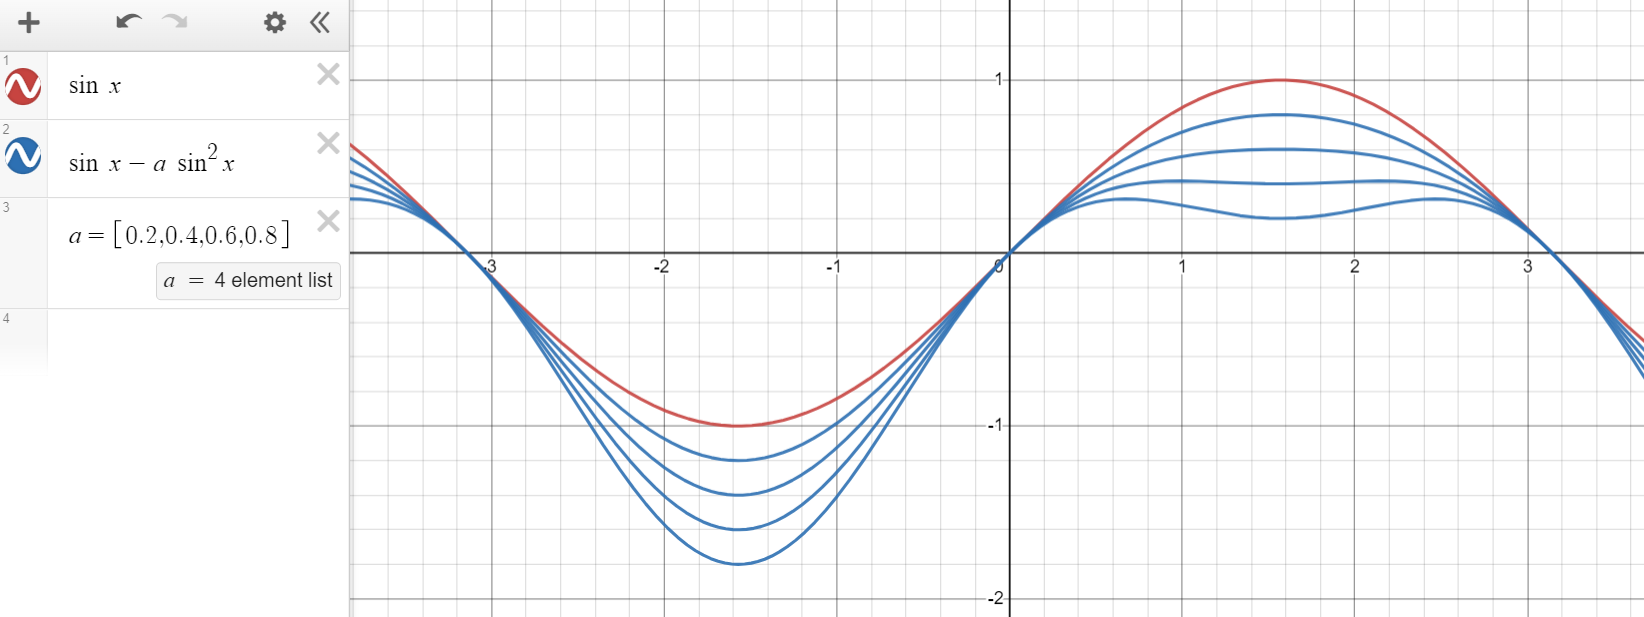
\includegraphics[scale=0.35]{sinx.png}
    \caption{$(\sin x)$ vs $(\sin x - a \sin^2 x)$}
\end{figure}

Let $f_a(x) = \sin x - a\sin^2 x$. If we are going to pretend $f_a(x)$ and $f(x)$ are polynomials, then we need to be including their non-real roots too. If we define $\sin x$ for $x \in \mathbb{C}$ as $\frac{e^{ix}-e^{-ix}}{2i}$ then $f(x) = \sin x$ still has only real roots but $f_a(x)$ has some additional non real roots (from solving $\sin x = 1/a$) that we need to have corresponding terms for in the partial fraction decomposition. In other words, when we say that there are no roots other than $n \pi$, that includes non-real roots. 

\begin{tcolorbox}
If \eqref{cosec} is correct, it seems to also imply that the exact shape of $\sin x$ is just the `right' shape for starting at $x=0$ with a slope of 1 and finishing at $x=\pi$ with a slope of -1, for example. If we try to do this by drawing any other shape there will apparently be some underlying non-real roots associated with it.
\end{tcolorbox}

To test our claim about taking into account the non-real roots of $f_a(x)$ too in the partial fraction decomposition, we calculate that these are of the form
\begin{align}
    x_k &= \alpha_k \mp i \beta && k \in \mathbb{Z} 
\end{align}
where
\begin{align}
    \alpha_k &= \frac{\pi}{2} + 2k\pi \\
    \beta &= \ln \left(\frac{1}{a} + \sqrt{\frac{1}{a^2} - 1}\right)
\end{align}
and
\begin{align}
    f_a'(x_k) = \mp i \sqrt{\frac{1}{a^2} - 1}
\end{align}
So the additional terms due to non real roots will be:
\begin{align}
    \frac{1}{\left(i\sqrt{\frac{1}{a^2}-1}\right) \left(x - (\alpha_k + i \beta)\right)} + \frac{1}{\left(-i\sqrt{\frac{1}{a^2}-1}\right) \left(x - (\alpha_k - i \beta)\right)} = \frac{\frac{2\beta a}{\sqrt{1-a^2}}}{x^2 + 2\alpha_k x + \alpha_k^2 + \beta^2}
\end{align}
And therefore we want to claim that:
\begin{align}
    \frac{1}{\sin x - a \sin^2 x} = \sum_{k = -\infty}^{\infty} \frac{(-1)^k}{x-k\pi} + \sum_{k = -\infty}^{\infty} \frac{\frac{2\beta a}{\sqrt{1-a^2}}}{x^2 + 2\alpha_k x + \alpha_k^2 + \beta^2}
\end{align}
I can't `prove' this equality but approximating finite sums on any graphing calculator can show us that they are close enough and so (probably) equal.

So, if it works for $\sin x$ then it probably works for some other simple functions too. If $f(x) = \tan x$ then $f$ is zero at only $n\pi$ (including possible non-real roots) for $n \in \mathbb{Z}$ and $f'(n\pi) = 1$. So
\begin{align}
    \frac{1}{\tan x} = \sum_{k = -\infty}^{\infty} \frac{1}{x-k\pi} \label{tan}
\end{align}
which is also \href{https://en.wikipedia.org/wiki/Trigonometric_functions#Partial_fraction_expansion}{true} and so is the case of $f(x) = \cos x$ and $f(x) = \cot x$ etc. Apparantly the discontinuity at $x = k\pi + \pi/2$ when treating $f(x) = \tan x$ as a polynomial does not break \eqref{tan}. The wikipedia example of $\csc^2 x$ suggests that the equations for the repeated roots case also hold for `non-polynomials'. I claim, without proof, that \eqref{basic} and \eqref{repeated} are awesome.

\end{document}
